\documentclass{standalone}
\usepackage{tikz}
\usetikzlibrary{patterns, positioning}


\begin{document}
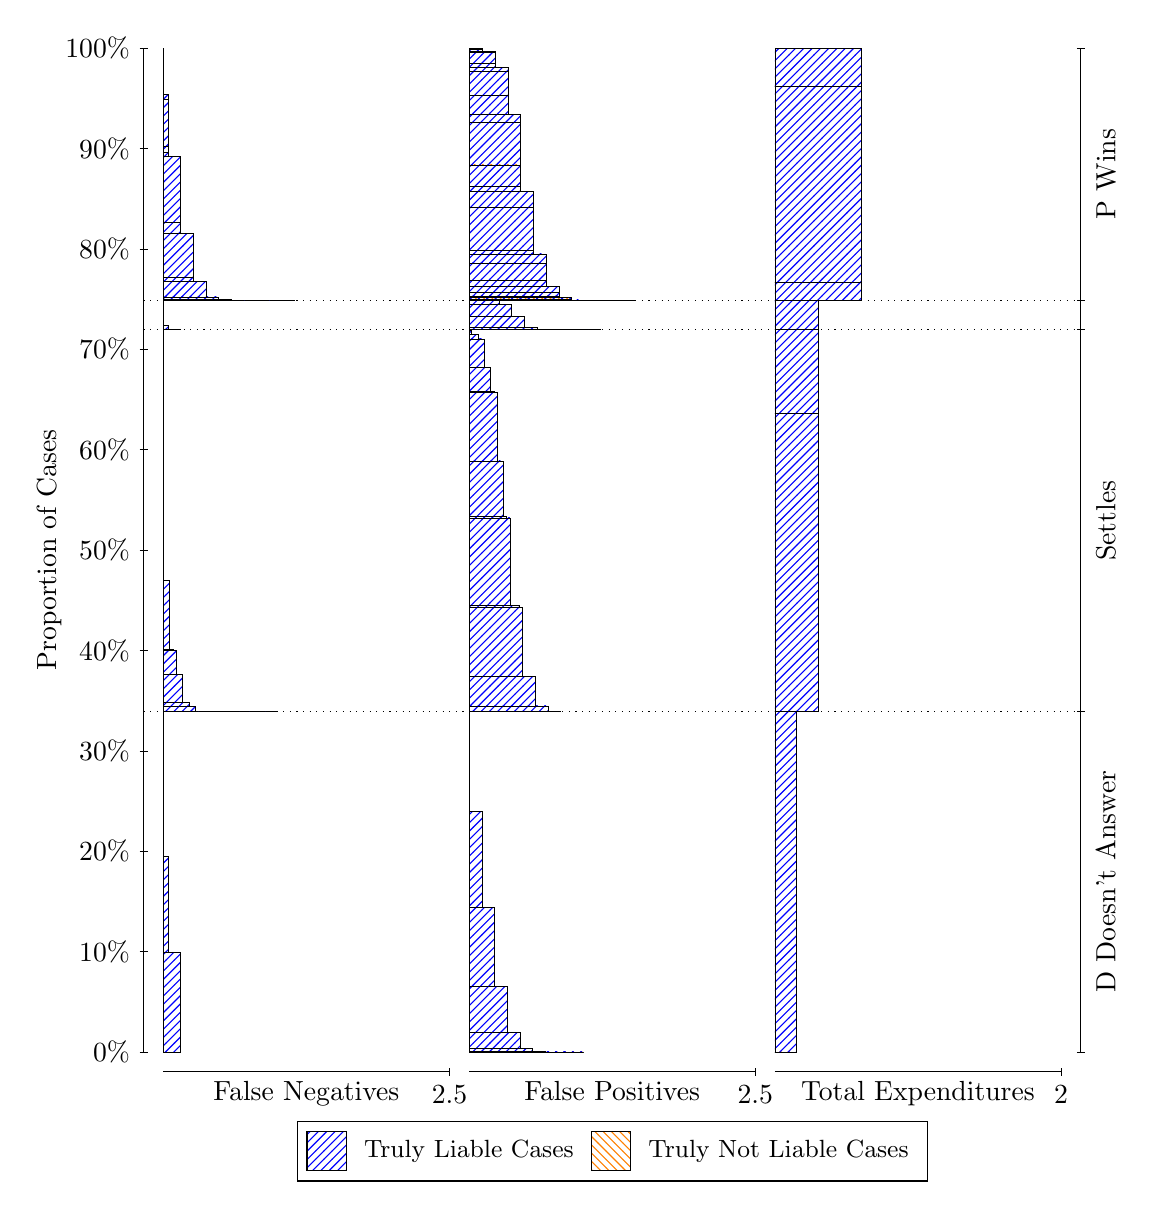
\begin{tikzpicture}
\draw[black, very thin] (1.5,1.75) -- (1.5,14.5);
\node[rotate=90, text=black, anchor=center] at (0.3, 8.125) {Proportion of Cases};
\draw[black, very thin] (1.45,1.75) -- (1.55,1.75);
\node[text=black, anchor=east] at (1.45, 1.75) {0\%};
\draw[black, very thin] (1.45,3.025) -- (1.55,3.025);
\node[text=black, anchor=east] at (1.45, 3.025) {10\%};
\draw[black, very thin] (1.45,4.3) -- (1.55,4.3);
\node[text=black, anchor=east] at (1.45, 4.3) {20\%};
\draw[black, very thin] (1.45,5.575) -- (1.55,5.575);
\node[text=black, anchor=east] at (1.45, 5.575) {30\%};
\draw[black, very thin] (1.45,6.85) -- (1.55,6.85);
\node[text=black, anchor=east] at (1.45, 6.85) {40\%};
\draw[black, very thin] (1.45,8.125) -- (1.55,8.125);
\node[text=black, anchor=east] at (1.45, 8.125) {50\%};
\draw[black, very thin] (1.45,9.4) -- (1.55,9.4);
\node[text=black, anchor=east] at (1.45, 9.4) {60\%};
\draw[black, very thin] (1.45,10.675) -- (1.55,10.675);
\node[text=black, anchor=east] at (1.45, 10.675) {70\%};
\draw[black, very thin] (1.45,11.95) -- (1.55,11.95);
\node[text=black, anchor=east] at (1.45, 11.95) {80\%};
\draw[black, very thin] (1.45,13.225) -- (1.55,13.225);
\node[text=black, anchor=east] at (1.45, 13.225) {90\%};
\draw[black, very thin] (1.45,14.5) -- (1.55,14.5);
\node[text=black, anchor=east] at (1.45, 14.5) {100\%};

\draw[black, very thin] (13.4,1.75) -- (13.4,14.5);
\draw[black, very thin] (13.35,1.75) -- (13.45,1.75);
\node[anchor=west] at (13.35, 1.75) {};
\draw[black, very thin] (13.35,6.0737) -- (13.45,6.0737);
\node[anchor=west] at (13.35, 6.0737) {};
\draw[black, very thin] (13.35,10.922) -- (13.45,10.922);
\node[anchor=west] at (13.35, 10.922) {};
\draw[black, very thin] (13.35,11.298) -- (13.45,11.298);
\node[anchor=west] at (13.35, 11.298) {};
\draw[black, very thin] (13.35,14.5) -- (13.45,14.5);
\node[anchor=west] at (13.35, 14.5) {};

\draw[black, very thin, pattern color=blue, pattern=north east lines] (1.75,1.75) rectangle (1.968,3.0179);
\draw[black, very thin, pattern color=blue, pattern=north east lines] (1.75,3.0179) rectangle (1.8065,4.2346);
\draw[black, very thin, pattern color=orange, pattern=north west lines] (1.75,4.2346) rectangle (1.75,4.2346);
\draw[black, very thin, pattern color=blue, pattern=north east lines] (1.75,4.2346) rectangle (1.75,6.0737);
\draw[black, very thin, pattern color=blue, pattern=north east lines] (1.75,6.0737) rectangle (3.2033,6.0737);
\draw[black, very thin, pattern color=blue, pattern=north east lines] (1.75,6.0737) rectangle (3.0419,6.0737);
\draw[black, very thin, pattern color=blue, pattern=north east lines] (1.75,6.0737) rectangle (2.8804,6.0737);
\draw[black, very thin, pattern color=blue, pattern=north east lines] (1.75,6.0737) rectangle (2.84,6.0737);
\draw[black, very thin, pattern color=blue, pattern=north east lines] (1.75,6.0737) rectangle (2.7189,6.0737);
\draw[black, very thin, pattern color=blue, pattern=north east lines] (1.75,6.0737) rectangle (2.6785,6.0737);
\draw[black, very thin, pattern color=blue, pattern=north east lines] (1.75,6.0737) rectangle (2.5574,6.0737);
\draw[black, very thin, pattern color=blue, pattern=north east lines] (1.75,6.0737) rectangle (2.517,6.0737);
\draw[black, very thin, pattern color=blue, pattern=north east lines] (1.75,6.0737) rectangle (2.4767,6.0737);
\draw[black, very thin, pattern color=blue, pattern=north east lines] (1.75,6.0737) rectangle (2.3959,6.0738);
\draw[black, very thin, pattern color=blue, pattern=north east lines] (1.75,6.0738) rectangle (2.3556,6.0738);
\draw[black, very thin, pattern color=blue, pattern=north east lines] (1.75,6.0738) rectangle (2.3152,6.0763);
\draw[black, very thin, pattern color=blue, pattern=north east lines] (1.75,6.0763) rectangle (2.2344,6.0787);
\draw[black, very thin, pattern color=blue, pattern=north east lines] (1.75,6.0787) rectangle (2.1941,6.0787);
\draw[black, very thin, pattern color=blue, pattern=north east lines] (1.75,6.0787) rectangle (2.1537,6.1346);
\draw[black, very thin, pattern color=blue, pattern=north east lines] (1.75,6.1346) rectangle (2.073,6.1882);
\draw[black, very thin, pattern color=blue, pattern=north east lines] (1.75,6.1882) rectangle (2.0326,6.1884);
\draw[black, very thin, pattern color=blue, pattern=north east lines] (1.75,6.1884) rectangle (1.9922,6.5498);
\draw[black, very thin, pattern color=blue, pattern=north east lines] (1.75,6.5498) rectangle (1.9115,6.8565);
\draw[black, very thin, pattern color=blue, pattern=north east lines] (1.75,6.8565) rectangle (1.8711,6.8617);
\draw[black, very thin, pattern color=blue, pattern=north east lines] (1.75,6.8617) rectangle (1.8307,7.7394);
\draw[black, very thin, pattern color=orange, pattern=north west lines] (1.75,7.7394) rectangle (1.75,7.7394);
\draw[black, very thin, pattern color=blue, pattern=north east lines] (1.75,7.7394) rectangle (1.75,10.922);
\draw[black, very thin, pattern color=blue, pattern=north east lines] (1.75,10.922) rectangle (1.968,10.928);
\draw[black, very thin, pattern color=blue, pattern=north east lines] (1.75,10.928) rectangle (1.8065,10.976);
\draw[black, very thin, pattern color=orange, pattern=north west lines] (1.75,10.976) rectangle (1.75,10.976);
\draw[black, very thin, pattern color=blue, pattern=north east lines] (1.75,10.976) rectangle (1.75,11.298);
\draw[black, very thin, pattern color=blue, pattern=north east lines] (1.75,11.298) rectangle (3.4213,11.298);
\draw[black, very thin, pattern color=blue, pattern=north east lines] (1.75,11.298) rectangle (3.2599,11.298);
\draw[black, very thin, pattern color=blue, pattern=north east lines] (1.75,11.298) rectangle (3.2599,11.298);
\draw[black, very thin, pattern color=blue, pattern=north east lines] (1.75,11.298) rectangle (3.0984,11.298);
\draw[black, very thin, pattern color=blue, pattern=north east lines] (1.75,11.298) rectangle (3.0984,11.298);
\draw[black, very thin, pattern color=blue, pattern=north east lines] (1.75,11.298) rectangle (2.9369,11.298);
\draw[black, very thin, pattern color=blue, pattern=north east lines] (1.75,11.298) rectangle (2.7754,11.298);
\draw[black, very thin, pattern color=blue, pattern=north east lines] (1.75,11.298) rectangle (2.7754,11.298);
\draw[black, very thin, pattern color=blue, pattern=north east lines] (1.75,11.298) rectangle (2.6139,11.303);
\draw[black, very thin, pattern color=blue, pattern=north east lines] (1.75,11.303) rectangle (2.4524,11.312);
\draw[black, very thin, pattern color=blue, pattern=north east lines] (1.75,11.312) rectangle (2.4524,11.339);
\draw[black, very thin, pattern color=blue, pattern=north east lines] (1.75,11.339) rectangle (2.291,11.54);
\draw[black, very thin, pattern color=blue, pattern=north east lines] (1.75,11.54) rectangle (2.1295,11.589);
\draw[black, very thin, pattern color=blue, pattern=north east lines] (1.75,11.589) rectangle (2.1295,12.142);
\draw[black, very thin, pattern color=blue, pattern=north east lines] (1.75,12.142) rectangle (1.968,12.286);
\draw[black, very thin, pattern color=blue, pattern=north east lines] (1.75,12.286) rectangle (1.968,13.122);
\draw[black, very thin, pattern color=blue, pattern=north east lines] (1.75,13.122) rectangle (1.8065,13.17);
\draw[black, very thin, pattern color=blue, pattern=north east lines] (1.75,13.17) rectangle (1.8065,13.254);
\draw[black, very thin, pattern color=blue, pattern=north east lines] (1.75,13.254) rectangle (1.8065,13.845);
\draw[black, very thin, pattern color=blue, pattern=north east lines] (1.75,13.845) rectangle (1.8065,13.912);
\draw[black, very thin, pattern color=orange, pattern=north west lines] (1.75,13.912) rectangle (1.75,13.912);
\draw[black, very thin, pattern color=blue, pattern=north east lines] (1.75,13.912) rectangle (1.75,14.5);
\draw[black, very thin, pattern color=orange, pattern=north west lines] (5.6333,1.75) rectangle (7.0867,1.75);
\draw[black, very thin, pattern color=blue, pattern=north east lines] (5.6333,1.75) rectangle (7.0867,1.75);
\draw[black, very thin, pattern color=blue, pattern=north east lines] (5.6333,1.75) rectangle (6.9252,1.75);
\draw[black, very thin, pattern color=blue, pattern=north east lines] (5.6333,1.75) rectangle (6.7637,1.7501);
\draw[black, very thin, pattern color=blue, pattern=north east lines] (5.6333,1.7501) rectangle (6.6022,1.7534);
\draw[black, very thin, pattern color=blue, pattern=north east lines] (5.6333,1.7534) rectangle (6.4407,1.7921);
\draw[black, very thin, pattern color=blue, pattern=north east lines] (5.6333,1.7921) rectangle (6.2793,1.9997);
\draw[black, very thin, pattern color=blue, pattern=north east lines] (5.6333,1.9997) rectangle (6.1178,2.5868);
\draw[black, very thin, pattern color=blue, pattern=north east lines] (5.6333,2.5868) rectangle (5.9563,3.5891);
\draw[black, very thin, pattern color=blue, pattern=north east lines] (5.6333,3.5891) rectangle (5.7948,4.8058);
\draw[black, very thin, pattern color=blue, pattern=north east lines] (5.6333,4.8058) rectangle (5.6333,6.0737);
\draw[black, very thin, pattern color=orange, pattern=north west lines] (5.6333,6.0737) rectangle (6.796,6.0737);
\draw[black, very thin, pattern color=blue, pattern=north east lines] (5.6333,6.0737) rectangle (6.796,6.0788);
\draw[black, very thin, pattern color=blue, pattern=north east lines] (5.6333,6.0788) rectangle (6.6345,6.1464);
\draw[black, very thin, pattern color=blue, pattern=north east lines] (5.6333,6.1464) rectangle (6.473,6.518);
\draw[black, very thin, pattern color=orange, pattern=north west lines] (5.6333,6.518) rectangle (6.4327,6.518);
\draw[black, very thin, pattern color=blue, pattern=north east lines] (5.6333,6.518) rectangle (6.4327,6.5243);
\draw[black, very thin, pattern color=blue, pattern=north east lines] (5.6333,6.5243) rectangle (6.3116,7.3951);
\draw[black, very thin, pattern color=blue, pattern=north east lines] (5.6333,7.3951) rectangle (6.2712,7.4187);
\draw[black, very thin, pattern color=blue, pattern=north east lines] (5.6333,7.4187) rectangle (6.1501,8.5323);
\draw[black, very thin, pattern color=blue, pattern=north east lines] (5.6333,8.5323) rectangle (6.1097,8.5564);
\draw[black, very thin, pattern color=orange, pattern=north west lines] (5.6333,8.5564) rectangle (6.0693,8.5564);
\draw[black, very thin, pattern color=blue, pattern=north east lines] (5.6333,8.5564) rectangle (6.0693,9.2562);
\draw[black, very thin, pattern color=blue, pattern=north east lines] (5.6333,9.2562) rectangle (5.9886,10.134);
\draw[black, very thin, pattern color=blue, pattern=north east lines] (5.6333,10.134) rectangle (5.9482,10.139);
\draw[black, very thin, pattern color=blue, pattern=north east lines] (5.6333,10.139) rectangle (5.9079,10.446);
\draw[black, very thin, pattern color=blue, pattern=north east lines] (5.6333,10.446) rectangle (5.8271,10.807);
\draw[black, very thin, pattern color=blue, pattern=north east lines] (5.6333,10.807) rectangle (5.7867,10.807);
\draw[black, very thin, pattern color=blue, pattern=north east lines] (5.6333,10.807) rectangle (5.7464,10.861);
\draw[black, very thin, pattern color=blue, pattern=north east lines] (5.6333,10.861) rectangle (5.6656,10.917);
\draw[black, very thin, pattern color=blue, pattern=north east lines] (5.6333,10.917) rectangle (5.6333,10.922);
\draw[black, very thin, pattern color=orange, pattern=north west lines] (5.6333,10.922) rectangle (7.3047,10.922);
\draw[black, very thin, pattern color=blue, pattern=north east lines] (5.6333,10.922) rectangle (7.3047,10.922);
\draw[black, very thin, pattern color=blue, pattern=north east lines] (5.6333,10.922) rectangle (7.1432,10.922);
\draw[black, very thin, pattern color=blue, pattern=north east lines] (5.6333,10.922) rectangle (6.9817,10.922);
\draw[black, very thin, pattern color=blue, pattern=north east lines] (5.6333,10.922) rectangle (6.8202,10.922);
\draw[black, very thin, pattern color=blue, pattern=north east lines] (5.6333,10.922) rectangle (6.6587,10.923);
\draw[black, very thin, pattern color=blue, pattern=north east lines] (5.6333,10.923) rectangle (6.4973,10.955);
\draw[black, very thin, pattern color=blue, pattern=north east lines] (5.6333,10.955) rectangle (6.3358,11.095);
\draw[black, very thin, pattern color=blue, pattern=north east lines] (5.6333,11.095) rectangle (6.1743,11.244);
\draw[black, very thin, pattern color=blue, pattern=north east lines] (5.6333,11.244) rectangle (6.0128,11.291);
\draw[black, very thin, pattern color=blue, pattern=north east lines] (5.6333,11.291) rectangle (5.8513,11.298);
\draw[black, very thin, pattern color=orange, pattern=north west lines] (5.6333,11.298) rectangle (7.7407,11.298);
\draw[black, very thin, pattern color=blue, pattern=north east lines] (5.6333,11.298) rectangle (7.7407,11.298);
\draw[black, very thin, pattern color=orange, pattern=north west lines] (5.6333,11.298) rectangle (7.5792,11.298);
\draw[black, very thin, pattern color=blue, pattern=north east lines] (5.6333,11.298) rectangle (7.5792,11.298);
\draw[black, very thin, pattern color=orange, pattern=north west lines] (5.6333,11.298) rectangle (7.4177,11.298);
\draw[black, very thin, pattern color=blue, pattern=north east lines] (5.6333,11.298) rectangle (7.4177,11.298);
\draw[black, very thin, pattern color=blue, pattern=north east lines] (5.6333,11.298) rectangle (7.4177,11.298);
\draw[black, very thin, pattern color=orange, pattern=north west lines] (5.6333,11.298) rectangle (7.2562,11.298);
\draw[black, very thin, pattern color=blue, pattern=north east lines] (5.6333,11.298) rectangle (7.2562,11.298);
\draw[black, very thin, pattern color=orange, pattern=north west lines] (5.6333,11.298) rectangle (7.0947,11.298);
\draw[black, very thin, pattern color=blue, pattern=north east lines] (5.6333,11.298) rectangle (7.0947,11.302);
\draw[black, very thin, pattern color=blue, pattern=north east lines] (5.6333,11.302) rectangle (6.9333,11.306);
\draw[black, very thin, pattern color=blue, pattern=north east lines] (5.6333,11.306) rectangle (6.9333,11.313);
\draw[black, very thin, pattern color=orange, pattern=north west lines] (5.6333,11.313) rectangle (6.9333,11.313);
\draw[black, very thin, pattern color=blue, pattern=north east lines] (5.6333,11.313) rectangle (6.9333,11.332);
\draw[black, very thin, pattern color=blue, pattern=north east lines] (5.6333,11.332) rectangle (6.7718,11.352);
\draw[black, very thin, pattern color=blue, pattern=north east lines] (5.6333,11.352) rectangle (6.7718,11.392);
\draw[black, very thin, pattern color=orange, pattern=north west lines] (5.6333,11.392) rectangle (6.7718,11.392);
\draw[black, very thin, pattern color=blue, pattern=north east lines] (5.6333,11.392) rectangle (6.7718,11.471);
\draw[black, very thin, pattern color=blue, pattern=north east lines] (5.6333,11.471) rectangle (6.6103,11.546);
\draw[black, very thin, pattern color=orange, pattern=north west lines] (5.6333,11.546) rectangle (6.6103,11.546);
\draw[black, very thin, pattern color=blue, pattern=north east lines] (5.6333,11.546) rectangle (6.6103,11.77);
\draw[black, very thin, pattern color=blue, pattern=north east lines] (5.6333,11.77) rectangle (6.6103,11.886);
\draw[black, very thin, pattern color=blue, pattern=north east lines] (5.6333,11.886) rectangle (6.4488,11.926);
\draw[black, very thin, pattern color=orange, pattern=north west lines] (5.6333,11.926) rectangle (6.4488,11.926);
\draw[black, very thin, pattern color=blue, pattern=north east lines] (5.6333,11.926) rectangle (6.4488,12.478);
\draw[black, very thin, pattern color=blue, pattern=north east lines] (5.6333,12.478) rectangle (6.4488,12.676);
\draw[black, very thin, pattern color=blue, pattern=north east lines] (5.6333,12.676) rectangle (6.2873,12.744);
\draw[black, very thin, pattern color=blue, pattern=north east lines] (5.6333,12.744) rectangle (6.2873,13.016);
\draw[black, very thin, pattern color=orange, pattern=north west lines] (5.6333,13.016) rectangle (6.2873,13.016);
\draw[black, very thin, pattern color=blue, pattern=north east lines] (5.6333,13.016) rectangle (6.2873,13.552);
\draw[black, very thin, pattern color=blue, pattern=north east lines] (5.6333,13.552) rectangle (6.2873,13.656);
\draw[black, very thin, pattern color=blue, pattern=north east lines] (5.6333,13.656) rectangle (6.1259,13.658);
\draw[black, very thin, pattern color=blue, pattern=north east lines] (5.6333,13.658) rectangle (6.1259,13.895);
\draw[black, very thin, pattern color=blue, pattern=north east lines] (5.6333,13.895) rectangle (6.1259,14.199);
\draw[black, very thin, pattern color=blue, pattern=north east lines] (5.6333,14.199) rectangle (6.1259,14.258);
\draw[black, very thin, pattern color=blue, pattern=north east lines] (5.6333,14.258) rectangle (5.9644,14.259);
\draw[black, very thin, pattern color=blue, pattern=north east lines] (5.6333,14.259) rectangle (5.9644,14.303);
\draw[black, very thin, pattern color=blue, pattern=north east lines] (5.6333,14.303) rectangle (5.9644,14.441);
\draw[black, very thin, pattern color=blue, pattern=north east lines] (5.6333,14.441) rectangle (5.9644,14.459);
\draw[black, very thin, pattern color=blue, pattern=north east lines] (5.6333,14.459) rectangle (5.8029,14.464);
\draw[black, very thin, pattern color=blue, pattern=north east lines] (5.6333,14.464) rectangle (5.8029,14.479);
\draw[black, very thin, pattern color=blue, pattern=north east lines] (5.6333,14.479) rectangle (5.8029,14.495);
\draw[black, very thin, pattern color=blue, pattern=north east lines] (5.6333,14.495) rectangle (5.6414,14.499);
\draw[black, very thin, pattern color=blue, pattern=north east lines] (5.6333,14.499) rectangle (5.6414,14.499);
\draw[black, very thin, pattern color=blue, pattern=north east lines] (5.6333,14.499) rectangle (5.6333,14.5);
\draw[black, very thin, pattern color=orange, pattern=north west lines] (9.5167,1.75) rectangle (9.7892,1.75);
\draw[black, very thin, pattern color=blue, pattern=north east lines] (9.5167,1.75) rectangle (9.7892,6.0737);
\draw[black, very thin, pattern color=orange, pattern=north west lines] (9.5167,6.0737) rectangle (10.062,6.0737);
\draw[black, very thin, pattern color=blue, pattern=north east lines] (9.5167,6.0737) rectangle (10.062,9.8595);
\draw[black, very thin, pattern color=orange, pattern=north west lines] (9.5167,9.8595) rectangle (10.062,9.8595);
\draw[black, very thin, pattern color=blue, pattern=north east lines] (9.5167,9.8595) rectangle (10.062,10.922);
\draw[black, very thin, pattern color=orange, pattern=north west lines] (9.5167,10.922) rectangle (10.062,10.922);
\draw[black, very thin, pattern color=blue, pattern=north east lines] (9.5167,10.922) rectangle (10.062,11.298);
\draw[black, very thin, pattern color=orange, pattern=north west lines] (9.5167,11.298) rectangle (10.607,11.298);
\draw[black, very thin, pattern color=blue, pattern=north east lines] (9.5167,11.298) rectangle (10.607,11.521);
\draw[black, very thin, pattern color=orange, pattern=north west lines] (9.5167,11.521) rectangle (10.607,11.521);
\draw[black, very thin, pattern color=blue, pattern=north east lines] (9.5167,11.521) rectangle (10.607,14.013);
\draw[black, very thin, pattern color=orange, pattern=north west lines] (9.5167,14.013) rectangle (10.607,14.013);
\draw[black, very thin, pattern color=blue, pattern=north east lines] (9.5167,14.013) rectangle (10.607,14.5);
\draw[black, dotted] (1.5,6.0737) -- (13.4,6.0737);
\draw[black, dotted] (1.5,10.922) -- (13.4,10.922);
\draw[black, dotted] (1.5,11.298) -- (13.4,11.298);
\draw[black, very thin] (1.75,1.5) -- (5.3833,1.5);
\node[text=black, anchor=north] at (3.5667, 1.5) {False Negatives};
\draw[black, very thin] (5.3833,1.45) -- (5.3833,1.55);
\node[text=black, anchor=north] at (5.3833, 1.45) {2.5};

\draw[black, very thin] (5.6333,1.5) -- (9.2667,1.5);
\node[text=black, anchor=north] at (7.45, 1.5) {False Positives};
\draw[black, very thin] (9.2667,1.45) -- (9.2667,1.55);
\node[text=black, anchor=north] at (9.2667, 1.45) {2.5};

\draw[black, very thin] (9.5167,1.5) -- (13.15,1.5);
\node[text=black, anchor=north] at (11.333, 1.5) {Total Expenditures};
\draw[black, very thin] (13.15,1.45) -- (13.15,1.55);
\node[text=black, anchor=north] at (13.15, 1.45) {2};

\node[text=black, centered, rotate=90] at (13.72, 3.9119) {D Doesn't Answer};
\node[text=black, centered, rotate=90] at (13.72, 8.4978) {Settles};

\node[text=black, centered, rotate=90] at (13.72, 12.899) {P Wins};

\draw (7.449999999999999,1.5) node[draw=none] (baseCoordinate) {};
\begin{scope}[align=center]
        \matrix[scale=0.5, draw=black, below=0.5cm of baseCoordinate, nodes={draw}, column sep=0.1cm]{
            \node[rectangle, draw, minimum width=0.5cm, minimum height=0.5cm, pattern color=blue, pattern=north east lines] {}; &
            \node[draw=none, font=\small, text=black] (B) {Truly Liable Cases}; &
            \node[rectangle, draw, minimum width=0.5cm, minimum height=0.5cm, pattern color=orange, pattern=north west lines] {}; &
            \node[draw=none, font=\small, text=black] (B) {Truly Not Liable Cases}; \\
            };
\end{scope}

\end{tikzpicture}
\end{document}